The weak phase \phis is an important parameter of the \BBbarSyst system. It is related to the third
type of \CP violation mentioned in \secref{Phenomenology}, namely in the interference between
the decay and mixing amplitudes, see \figref{interference}. In the current section \phis and
its relevance to the search for new particles is discussed.

\newcommand{\ffig}{f}
% \newcommand{\phimixfig}{\phi_\text{mix}}
% \newcommand{\phifig}{\phi_\text{dec}}
% \newcommand{\phibarfig}{\kern 0.15em \overline{\kern -0.15em \phi_\text{dec} \kern -0.60em} \kern 0.60em}
\begin{figure}[h]
  \centering
  \resizebox{0.4\textwidth}{!}{\begin{picture}(0,0)%
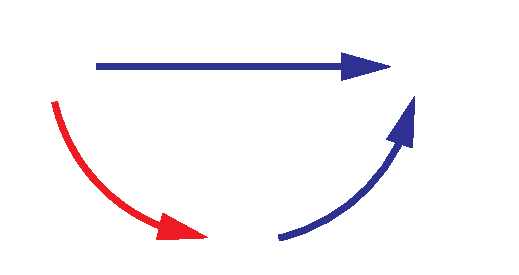
\includegraphics{Figures/Chapter1/decay_CMYK.pdf}%
\end{picture}%
\setlength{\unitlength}{4144sp}%
%
\begingroup\makeatletter\ifx\SetFigFont\undefined%
\gdef\SetFigFont#1#2#3#4#5{%
  \reset@font\fontsize{#1}{#2pt}%
  \fontfamily{#3}\fontseries{#4}\fontshape{#5}%
  \selectfont}%
\fi\endgroup%
\begin{picture}(3939,2094)(2644,-2188)
\put(3286,-736){\makebox(0,0)[rb]{\smash{{\SetFigFont{25}{30.0}{\sfdefault}{\mddefault}{\updefault}{\color[rgb]{0,0,0}$\Bs$}%
}}}}
\put(5761,-736){\makebox(0,0)[lb]{\smash{{\SetFigFont{25}{30.0}{\sfdefault}{\mddefault}{\updefault}{\color[rgb]{0,0,0}$\ffig$}%
}}}}
\put(4501,-421){\makebox(0,0)[b]{\smash{{\SetFigFont{25}{30.0}{\sfdefault}{\mddefault}{\updefault}{\color[rgb]{0,0,1}}%
}}}}
\put(5581,-1771){\makebox(0,0)[lb]{\smash{{\SetFigFont{25}{30.0}{\sfdefault}{\mddefault}{\updefault}{\color[rgb]{0,0,1}}%
}}}}
\put(3331,-1771){\makebox(0,0)[rb]{\smash{{\SetFigFont{25}{30.0}{\sfdefault}{\mddefault}{\updefault}{\color[rgb]{1,0,0}}%
}}}}
\put(4501,-2041){\makebox(0,0)[b]{\smash{{\SetFigFont{25}{30.0}{\sfdefault}{\mddefault}{\updefault}{\color[rgb]{0,0,0}$\Bsb$}%
}}}}
\end{picture}%
}
  \caption{The two interfering decay paths leading to the same final state.}
  \label{interference}
\end{figure}

The parameter \phis manifests itself in the time dependence of the so called $\bquark \rightarrow \cquark\cquarkbar\squark $ transitions.
An example of the latter is shown in \figref{bs2jpsiphi}. In addition, the final state of the \Bs meson has to be
a \CP eigenstate, which implies that both \Bs and \Bsb can decay into it, such that the two decay paths
illustrated in \figref{interference} can interfere with each other.

\begin{figure}[!h]
  \centering
  {\sffamily \input{Figures/Chapter1/tree}}
  \caption{Leading order tree diagram of the \BsJpsiPhi decay.}
  \label{bs2jpsiphi}
\end{figure}

A common way to parameterize \CP violation in the interference between mixing and decay is:

\begin{equation}
  \centering
  \lambda_{f} = \frac{q}{p} \frac{\bar{A}_f}{A_f}. % \equiv \left|\lambda_f\right| e^{i\phis}.
\label{lambda_cpv}
\end{equation}

\noindent Note that $\lambda_f$ is not to be confused with the $\lambda$ of the Wolfenstein parametrization.
Assuming no \CP violation in either \BBbarSyst mixing or in the decay to the \CP eigenstate $f$, the asymmetry
associated to the interference can be written as:

\newcommand{\half}{\frac{1}{2}}
\begin{equation}
  \centering
  a_{\CP}^{\rm interf}(t) = \frac{ - \Im(\lambda_f) \sin(\Delta m_s t)} {\cosh(\half \Delta\Gamma_s t) - \Re(\lambda_f)\sinh(\half\Delta\Gamma_s t)}.
\label{cpv_interf}
\end{equation}

\noindent It can be seen that the previous asymmetry shows an oscillatory behaviour versus time, due
to the presence of the $\sin(\Delta m_s t)$ term. The frequency of the oscillation is driven by $\Delta m_s$, whereas
the amplitude is proportional to $\Im\lambda_f$.

For completeness, according to \cite{DeBruyn-thesis,jeroenThesis}, the parameter $\lambda_f$ is also related to the $\Acp{\rm dir}$ as well as to two
other types of asymmetries. The asymmetries are shown in \equref{cp_asym_lambda} and they come from the differential decay rate equations of the $\Bs\to f$
 and $\Bsb\to f$.

\begin{equation}
  \centering
  \Acp{\rm dir}      \equiv \frac{ 1-|\lambda_f|^2} {1 + |\lambda_f|^2},\;\;\;\;\;
  \Acp{\rm mix}      \equiv \frac{ 2 \Im\lambda_f} {1 + |\lambda_f|^2},\;\;\;\;\;
  \Acp{\Delta\Gamma} \equiv \frac{ 2 \Re\lambda_f} {1 + |\lambda_f|^2}.
\label{cp_asym_lambda}
\end{equation}

\noindent The second asymmetry, \Acp{\rm mix}, expresses the mixing induced \CP asymmetry, whereas \Acp{\Delta\Gamma} is associated with the
difference in the decay rate of the mass eigenstates of \equref{bs_mass_eigen}.

It is interesting to point out that according to \equref{cpv_interf} and \equref{cp_asym_lambda} \CP asymmetry
can still be observed in the interference between decay and
mixing even if no \CP violation occurs in either the mixing or decay. This is possible if the imaginary part,
$\Im\lambda_f$, in \equref{lambda_cpv} is not zero. The asymmetry of \equref{cpv_interf} can vanish at a
particular point of time or for a given time interval. Because of that \equref{cpv_interf} should not
be integrated over time when measuring \phis. This implies that this asymmetry should be measured as
a function of the {\it decay time} of the \Bs (\Bsb) meson. Where decay time is the time interval between
the production and decay of a particle, for example the \Bs particle.

The imaginary part of \equref{lambda_cpv} can be expressed as a combination of CKM elements, given a certain final state $f$, like $\jpsi\Pphi$.
Under the assumption that for this final state only the leading order diagrams of \figref{bs_box} and \figref{bs2jpsiphi} contribute to the
the \BBbarSyst mixing and decay respectively; Then the leading order Standard Model estimate of $\Im(\lambda_f)$ is written as:

\begin{equation}
  \centering
 \Im(\lambda_f) = \Im\parenthesis{ \frac{\Vts\Vtb^*}{\Vts^*\Vtb} \; \Vcs^*\Vcb \; \frac{1}{\Vcs\Vcb^*} },
 \label{lambdaf_ckm}
\end{equation}

\noindent where the first fraction is related to the mixing part \qoverp whereas the second and third come from
the \Bsb and \Bs decay amplitudes. Note that the \tquark quark dominates the loop in \figref{bs_box} over the
\cquark and \uquark quarks. Re-writing the imaginary part of \equref{lambdaf_ckm} taking into account
\equref{ckm_angles_def}, one can obtain:

\begin{equation}
  \centering
  \Im\parenthesis{ \brackets{ \frac{\Vts\Vtb^*}{\Vcs\Vcb^*}}^2 } =
  \sin \parenthesis{2 \arg \parenthesis{\frac{\Vts\Vtb^*}{\Vcs\Vcb^*}}} =
  \sin \parenthesis{-2\betas}.
 \label{lambda_ckm_manip}
\end{equation}

\noindent The parameter \phis is finally defined as:

\begin{equation}
  \centering
  \phis\equiv-2\betas.
 \label{phis_def}
\end{equation}

\noindent Lastly, an implication arises from the choice of the intermediate resonances, $\jpsi$ and $\Pphi$,
which both have a non-zero spin quantum number. Specifically, the sum of the $\jpsi$ and $\Pphi$ spin vectors
has to be compensated by orbital angular momentum, $l$, such that the $\jpsi\Pphi$ state has a zero total
angular momentum, matching the total angular momentum of the initial \Bs meson (angular momentum conservation is implied).
As a result, the presence of orbital angular momentum makes it such that the $\jpsi\Pphi$ is not a pure \CP-eigenstate,
but rather an admixture of a \CP-odd and \CP-even components. Thus, for a particular $\jpsi\Pphi$ decay the value of
the total angular momentum, $l$, dectates wheather the \CP eigenvalue of the previous decay is \CP-odd or \CP-even:

\begin{equation}
  \centering
  \CP\ket{\jpsi\Pphi} = (-1)^l\ket{\jpsi\Pphi}.
 \label{cp_eigenstates}
\end{equation}

\noindent As a consequence \equref{lambda_ckm_manip} needs to be modified as:

\begin{equation}
  \centering
  \sin \parenthesis{-2\betas} \to (-1)^l \sin \parenthesis{-2\betas}
 \label{phis_def}
\end{equation}

It turns out that in order to properly measure \phis it is necessary to disentangle the \CP-odd and \CP-even
components by means of an angular analysis of \BsJpsiPhi decays. The angular analysis is based on the
angular distributions of \phiKK and \Jpsimumu, see \secref{Diferential_Decay_Rate} for the angular analysis
of \BsJpsiKst decays.

\subsection{Measuring $\boldsymbol{\phis}$}
\label{measuring_phis}

The parameter \phis has been measured at the \lhcb experiment by studying the decays of \BsJpsiPhi \cite{phis-3fb-paper}.
The particular choice of the final state, where \phiKK and \Jpsimumu, is preferred for several reasons. First the large number
of selected \BsJpsiPhi decays available at \lhcb, roughly $90$k at the end of the \runtwo is an advantage. Second, it is relatively
easy to select $\Pphi$ over other mesons that decay to a $\Kp\Km$ pair. This is due to the fact that the $\Pphi$ meson resonance dominates
the $\Kp\Km$ mass distribution within a window of about $\pm 60 \mevcc$ around its mass. This allows for the analysis to be
almost independent of the \mKK mass variable simplifying the procedure. However an angular analysis is necessary
to disentangle the odd and even \CP components of the final state $\jpsi\Pphi$.
In addition, as it was already implied \phis can be correctly probed only when the decay time dependence of the \BsJpsiPhi decays is taken into
account. Furthermore knowledge on whether the final state $\jpsi\Pphi$ originated from a \Bs or a \Bsb is necessary since it
significantly improves the sensitivity of the \phis measurement. The technique used to deduce this information is called {\it flavor tagging}
and it complicates the analysis further. On top of that experimental effects such as angular and time efficiencies plus modeling the
\lhcb detector's time resolution need to be taken into account.

\begin{figure}[h]
  \centering
    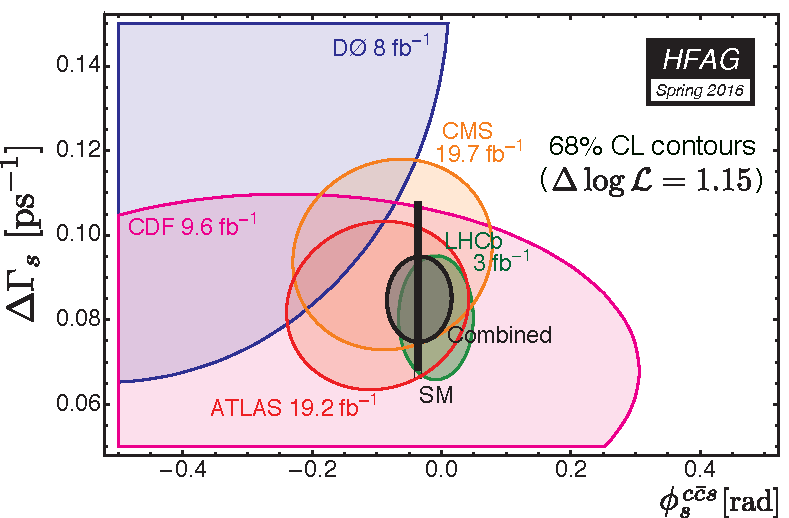
\includegraphics[trim=0cm 0cm 0cm 0cm, clip=true, scale=0.8]{Figures/Chapter1/hfag_Spring2016_DGsphis_zoom.pdf}
    \caption{Likelihood contours of $\Delta\Gamma_s-\phis$ (here $\phis\equiv \phis^{c\bar{cs}}$). Many individual measurements are
             combined to the black ellipse. Standard Model prediction is represented by the black band. The \lhcb measurement
             mentioned in \equref{phis_lhcb} is illustrated by the green ellipse. The combined measurements agree with the Standard Model
             predictions. Plot from \cite{hfag-2014} }
    \label{hfag_phis_dg}
\end{figure}

The status of the \phis measurements is shown in \figref{hfag_phis_dg}, where \lhcb has the most precise measurement to date.
The combined \phis value from \lhcb \cite{phis-3fb-paper}, shown in \equref{phis_lhcb}, includes two chanells \BsJpsiPhi and \BsJpsipipi:

\begin{subequations}
  \label{phis_lhcb_theo}
  \begin{align}
  \centering
  \phiS{\lhcb}           &=  -0.010 \pm 0.039(\text{total})  \;\; \text{rad},
  \label{phis_lhcb}\\
  \phiS{SM,tree}  &= -0.03761 {}^{+0.00073}_{-0.00082}  \;\; \text{rad}.
  \label{phis_theo}
\end{align}
\end{subequations}

\noindent The previous result is consistent with global fits to the Standard Model parameters
\equref{phis_theo} \cite{ckm-fitter-phis-pred} (updated with summer the 2015 result), within the current experimental uncertainty.

\subsection{Probing New Physics}
\label{probe_new_phys}

As explained at the end of \secref{The_Standard_Model} it seems that the Standard Model needs to be extended
to describe effects and phenomena beyond our current theoretical framework. In the majority of the Standard Model
extensions some new particle (field) is introduced. For example {\it Supersymmetry} \cite{Golfand:1971iw,Volkov:1973ix,Wess:1974tw}
doubles the number of elementary particles by predicting a supersymmetric partner for each one of them.
Supersymmetry is appealing since it could solve important problems such as the {\it hierarchy problem}
related to the value of the Higgs boson mass.

There are typically two ways that these particles are sought for, namely {\it on-shell} and {\it off-shell}.
The first implies that the particle is created in high energy collisions and its presence is inferred by detecting the products of
its decay. A typical example is the recent discovery of the Higgs boson at \lhc \cite{higgs-cms,higgs-atlas}.
In the second scenario the presence of a new particle modifies some observable quantity, like $\phis$, in such a way that Standard Model
cannot explain. In that case it is not necessary for this particle to be created in the first place.
One of the most significant examples of this type is the existence of the \tquark quark, whose large mass
drastically affects the \BdBdbarSyst oscillation frequency \cite{argus-bbmix}. The second approach is the one
that is followed in flavor physics.

Particularly, in the case of \BsJpsiPhi decays, the predicted Standard Model value of \equref{phis_theo} is precise enough
such that the presence of new particles could shift its value \cite{Buras:2009if,Chiang:2009ev,Datta:2009fk} significantly.
Any deviation (small or large) is a direct evidence for physics beyond the Standard Model, making \phis an excellent observable for probing NP.
This situation is shown in \equref{phis_meas} where the measured value \phiS{eff} is interpreted
as the sum of the Standard Model prediction $\phiS{SM}$ and the introduced from New Physics shift $\Delta\phiS{NP}$.

\begin{equation}
  \centering
 \phis^{\text {eff}} = \phis^{\tiny \text{SM}} + \Delta\phiS{NP}.
 \label{phis_meas}
\end{equation}

In view of the combined \phis result illustrated in \figref{hfag_phis_dg} New Physics effects, if there in the first place, must be small.
This is supported by other interesting measurements of flavor physics observables where deviations from Standard Model are not significant enough
to claim the presence of New Physics effects. Such hints come from the rare decays \Bsmm, \Bdmm \cite{CMS:2014xfa} and $\BdKstmumu$\cite{Aaij:2015oid}
or from the $\mathcal{R}\left(\Dstar\right)$ measurement \cite{Aaij:2015yra}.
An interesting fact that could be helpful in the future is that all these deviations and tensions are
correlated with each other. This implies that under the assumption of a certain New Physics model all the flavor physics
observables need to form a coherent picture such that the assumed model can be identified.
The latter points out the power of flavor physics observables.

Lastly, the smallness of New Physics hints compels the scientific community to continue measuring the
flavor physics observables with increased precision, both from the theory and the experimental side.
However, in this precision era higher order effects become important and need to be taken into account,
as explained in the following subsection. Given that, \phis will most likely continue to play an important
role in the pursuit for New Physics.

\subsection{Higher Order Effects in $\boldsymbol{\phis}$}
\label{TheBsJpsiKstDecay}
As mentioned in \secref{WeakPhase} \BsJpsiPhi decays are dominated by the tree diagram of \figref{bs2jpsiphi}.
However the decay also receives contributions from higher order suppressed process, for example the so called
{\it penguin} diagrams (or topologies) shown in \figref{bs2jpsiphi_peng}. The \phis measurement of \equref{phis_lhcb}
ignores the contribution of these penguin diagrams. This has been a reasonable assumption before the \lhcb measurement
which showed that the measured \phiS{eff} value is consistent with the Standard Model prediction \phiS{SM,tree},
within the current experimental accuracy.

\begin{figure}[h]
  \centering
  {\sffamily %%BoundingBox: -5 0 121 170
%%HiResBoundingBox: -5 0 120.57008 169.36447

\begin{fmffile}{Figures/Chapter1/penguin}
  \fmfframe(17,-25)(31,-25){
    \begin{fmfgraph*}(115,170)
      \fmfstraight
      \fmfleft{i0,i1,i2,i3,i4,i5}
      \fmfright{o0,o1,o2,o3,o4,o5}
      \fmf{fermion,tension=1.8,label.side=left,label=b}{v5,i3}
      \fmf{fermion,tension=1.5,right=0.2,label.side=left,label={\hspace*{18pt}u,,c,,t}}{v2,v5}
      \fmf{gluon,tension=2}{v4,v2}
      \fmf{dbl_dashes,tension=0}{v4,v2}
      \fmf{fermion,tension=0.3,right=0.2,label.side=left }{v3,v2}
      \fmf{boson,tension=0.6,left=0.3,label=W$^+$,label.side=left}{v3,v5}
      \fmf{fermion,label=c,tension=0.9,right=0.3,label.side=left}{o4,v4}
      \fmf{fermion,label=c,tension=0.9,right=0.3,label.side=left}{v4,o3}
      \fmf{fermion,label=s,label.side=left}{o2,v3}
      \fmffreeze
      \fmf{fermion,tension=0.7,label=s,label.side=left}{v1,o1}
      \fmf{fermion,tension=1,label.side=left,label=s}{i2,v1}
      %\fmf{phantom,tension=0.4}{v4,v1}
      \fmf{phantom,tension=0.4}{v3,v1,v5}
      \fmf{plain,right=0.2}{i2,i3}
      \fmf{plain,left=0.2,label=$\Bs$}{i2,i3}
      \fmf{plain,right=0.2,label=$\phi$}{o1,o2}
      \fmf{plain,left=0.2}{o1,o2}
      \fmf{plain,right=0.2,label=$\jpsi$}{o3,o4}
      \fmf{plain,left=0.2}{o3,o4}
    \end{fmfgraph*}
  }
\end{fmffile}
}
  \caption{ Higher order-penguin diagram. This diagram is suppressed as explained in \secref{Penguins}.}
  \label{bs2jpsiphi_peng}
\end{figure}

However, with the increasing accuracy at the \lhcb experiment the previous assumption needs to be revisited.
Specifically, because of the fact that penguin topology contributions shifts the leading tree level Standard Model prediction.
This shift could be misinterpreted as $\Delta\phiS{NP}$ if these penguin contributions are not properly estimated.
Thus in order to correctly probe New Physics in future measurements the penguin topology contributions $\Delta\phiS{SM,peng}$
have to be estimated. The above situation is spelled out as:

\begin{equation}
\centering
 \phis^{\text {eff}} = \phis^{\tiny \text{SM,tree}} + \Delta\phiS{SM,peng} + \Delta\phis^{\tiny \text{NP}}.
 \label{phis_sm_peng}
\end{equation}

\noindent Calculations for the penguin contributions to $\Delta\phiS{SM,peng}$ are available \cite{Liu:2013nea,Frings:2015eva}.
However, these calculations are not precise enough, since they involve non-perturbative long-distance QCD effects. Thus an alternative
approach, according to \cite{DeBruyn:2014oga,Frings:2015eva,Faller:2008gt,Liu:2013nea,DeBruyn-thesis}, is followed in order to experimentally
determine $\Delta\phiS{SM,peng}$ by relying to similar decay channels as \BsJpsiPhi as well. By doing so the precision on the penguin
contributions increases. A description of the necessary formalism to determine the penguin shift, $\Delta\phiS{SM,peng}$, using also the
channels \BsJpsiKst and \BsJpsiRho is given in \chapref{Penguins}.
